\documentclass{rapportCS}
\usepackage{lipsum}
\title{Rapport CentraleSupelec - Template} %Titre du fichier

%%%%%%%%%%%%%%%%%%%%%% LES PACKAGES
%-------------------
% gestion des pages
%-------------------
\usepackage{pdflscape} %pages horizontales dans le PDF
\usepackage{calc} %pour pouvoir écrire \textwidth-1cm


%-------------------
% sommaire 
%-------------------
\usepackage{tocloft}%mise en forme de la toc
\usepackage{titlesec}%mise en forme des titres de section
\usepackage[nottoc, notlof, notlot]{tocbibind}


%-------------------
% langue et encodage
%-------------------
\usepackage[utf8]{inputenc}
\usepackage[T1]{fontenc}
\usepackage[]{babel}
%\usepackage[english]{babel}
%\usepackage[french]{babel}


%-------------------
% symboles et mode maths
%-------------------
\usepackage{amsmath,amsfonts,amssymb}
\usepackage{textcomp,lmodern}%pour l'euro
\usepackage{mathrsfs}%lettres style manuscrit italique


%-------------------
% code
%-------------------
\usepackage{minted}
%%-- pour la commande qui évite l'italique
%%-- voir https://github.com/gpoore/minted/issues/71
%\usepackage{etoolbox}
%\usepackage{newunicodechar}
\usepackage[vlined, french, onelanguage]{algorithm2e}



%-------------------
% environnement, théorèmes et exercices
%-------------------
%\usepackage{thmbox}%pour les jolis thm


%-------------------
% tableaux
%-------------------
\usepackage{array,multirow}


%-------------------
% images
%-------------------
\usepackage{xcolor} %pour redefinir des couleurs
\usepackage{caption}%les personaliser (les centrer par ex)
\usepackage{graphicx} % pour includegraphics

\usepackage{tikz} %graphiques et dessins
\usetikzlibrary{shapes}%pr écrire \node[ellipse] par ex
\usetikzlibrary{positioning} %pr écrire \node[below rigth = 3pt and 5pt]
\usetikzlibrary{decorations.pathreplacing}%pr les accolades
\usetikzlibrary{patterns}%pour les hachures





%-------------------
% divers
%-------------------
\usepackage{cancel}%pour barrer
%-------------------
\usepackage{lipsum}% for dummy text
%-------------------
\usepackage{appendix}%pour les annexes




%%%%%%%%%%%%%%%%%%%%%% MISE EN FORME
\input{mise_en_forme.tex}

%%%%%%%%%%%%%%%%%%%%%%% LA PALETTE DE COULEURS
%%%%%%%%%%%%%% couleurs locales
\definecolor{jaune}{RGB}{255, 195, 0 }
\colorlet{oranger}{orange!50!jaune}
\definecolor{orange}{RGB}{250, 130, 1}

\definecolor{vert}{RGB}{194, 247, 50}
\definecolor{herbe}{RGB}{80, 180, 33}
\definecolor{vertFonce}{RGB}{20, 148, 20} 

\colorlet{vertdEau}{blue!50!green!30!white} 
\definecolor{turquoise}{RGB}{0, 204, 203}
\colorlet{monCyan}{turquoise!90!blue} 
\definecolor{turquoiseFonce}{RGB}{0, 149, 182} 
\colorlet{marine}{blue!60!black}
\colorlet{doubleu}{gray!50!blue}


\colorlet{lavande}{vertdEau!50!blue}
\definecolor{mauve}{RGB}{161, 132, 220}
\definecolor{lilas}{RGB}{154, 107, 165}


\definecolor{prunelle}{RGB}{106,24, 141}
\definecolor{prune}{RGB}{121, 7, 123}
\definecolor{violet}{RGB}{153, 0, 139}
\definecolor{violette}{RGB}{128, 0, 128} 

\definecolor{roseAcidule}{RGB}{255, 0, 127} 
\colorlet{rose}{orange!50!oranger!50!magenta!50!violet}
\definecolor{grenat}{RGB}{141, 24, 59}
\colorlet{framboise}{magenta!90!red!80!black}




\colorlet{ocre}{orange!90!green!80!white} 
\definecolor{chamois}{RGB}{200, 141, 75}

\definecolor{briqueRouge}{RGB}{200, 48, 24}
\definecolor{brique}{RGB}{141, 48, 24}
\definecolor{taupe}{RGB}{165, 137, 107}


\colorlet{expli}{gray}


\colorlet{saumon}{yellow!45!magenta}



%%%%%%%%%%%%%%%%%%%%%%% LES COMMANDES 
%%%%%%%%%%%%%%%%%%%%%%%%%%%%%%%%%%%%%%%%%%%%
% GENERAL  
%%%%%%%%%%%%%%%%%%%%%%%%%%%%%%%%%%%%%%%%%%%%

%raccourcis généraux
\newcommand {\ie}{\textit{i.e}. }
\newcommand {\cf}{\textit{Cf.} }
\newcommand {\resp}{resp.\! }


%pour les belles fonctions (à mettre entre $ $  ou entre $$ $$ )
\newcommand{\fonction}[5]{ 
#1 =
\left( \! \begin{tabular}{c@{ }c@{ }l} 
$#2$  & $\longrightarrow$   & $#3$  \\
$#4$  & $\longmapsto$       & $#5$ 
\end{tabular} \! \right)
}

%le widebar (inutile si package mathabx
\newcommand{\widebar}[1]{\overline{#1}}

%symboles rapprochés
\renewcommand {\=}{\!=\!}
\renewcommand {\-}{\!-\!}
\renewcommand {\:}{\!:\!}
\newcommand {\+}{\!+\!}
\newcommand {\iin}{\!\in\!}
\newcommand {\inclus}{\!\subseteq\!}

%symboles
\newcommand{\bubullet}{-}
\newcommand{\subbullet}{\circ}
\newcommand{\parties}{\mathcal{P}}

%produit scalaire
\renewcommand{\.}{\!\cdot\!}

%indicatrice
\newcommand{\1}{\mathbb{I}}

%cardinal
\newcommand{\card}[1]{\left|#1\right|}

%%%%%%%%%%%%%%%%%%%%%%%%%%%%%%%%%%%%%%%%%%%%
% ENSEMBLES DE NOMBRES & ESPACES DE VARIABLES  
%%%%%%%%%%%%%%%%%%%%%%%%%%%%%%%%%%%%%%%%%%%%

%pour N,Z,R 
\newcommand {\NN}{\mathbb{N}}
\newcommand {\NNe}{\NN^*}
\newcommand {\R}{\mathbb{R}}
\newcommand {\Rp}{\R_+}
\newcommand {\Rpe}{\R^*_+}
\renewcommand {\Re}{\R^*}
\newcommand {\Z}{\mathbb{Z}}


%%%%%%%%%%%%%%%%%%%%%%%%%%%%%%%%%%%%%%%%%%%%
% LES NOUVEAUX OPERATEURS  
%%%%%%%%%%%%%%%%%%%%%%%%%%%%%%%%%%%%%%%%%%%%

%optim
\DeclareMathOperator*{\argmin}{arg\,min}
\DeclareMathOperator*{\argmax}{arg\,max}

%analyse cvx
\DeclareMathOperator*{\conv}{conv}
\DeclareMathOperator*{\extr}{extr}
\DeclareMathOperator*{\vect}{vect}
\DeclareMathOperator*{\aff}{aff}





%%%%%%%%%%%%%%%%%%%%%%%%%%%%%%%%%%%%%%%%%%%%
% ICONES ET SYMBOLES HORS MATHS 
%%%%%%%%%%%%%%%%%%%%%%%%%%%%%%%%%%%%%%%%%%%%
\newcommand{\flch}{\item[$\rightarrow$]}

\newcommand{\attention}{\dbend}

\newcommand{\alamain}{{\LARGE\ding{45}}}

\newcommand{\surmachine}{

\begin{tikzpicture}[scale=0.1]
\draw[line width=1.2pt](-2,0) rectangle (2,3);
\fill(-1,0)--(1,0)--(2,-1)--(-2,-1)--(-1,0);
\end{tikzpicture}
}

\newcommand{\pasapas}{
\begin{tikzpicture}[scale=0.1]
\draw (0,0)--(0,1)--(1,1)--(1,2)--(2,2)--(2,3)--(3,3)--(3,4)--(4,4)--(5,4)--(5,0)--(0,0);
\end{tikzpicture}
}

\newcommand{\afaire}{
\begin{tikzpicture}[scale=0.1]
\draw (0,0)rectangle(4,4);
\end{tikzpicture}
}

\newcommand{\uneetoile}{{\LARGE$*$}\,}
\newcommand{\deuxetoiles}{{\LARGE$*\,*$}\,}
\newcommand{\troisetoiles}{{\LARGE$_*^*$}{\large$*$}\,}


\newcommand{\couleur}[1]{\textcolor{turquoiseFonce!70!black}{#1}}
\newcommand{\important}[1]{\textbf{\couleur{#1}}}

\newtcolorbox{coder}{
enhanced,
boxrule=0pt,frame hidden,
borderline west={4pt}{0pt}{briqueRouge},
colback=black!3!white,
sharp corners
}
\newtcolorbox{codeb}{
enhanced,
boxrule=0pt,frame hidden,
borderline west={4pt}{0pt}{vertdEau},
colback=black!3!white,
sharp corners
}

\newcommand{\intervalle}[2]{[\![#1,#2]\!]}

\renewcommand{\appendixpagename}{Annexes}
\renewcommand{\appendixtocname}{Annexes}
%%%%%%%%%%%%%%%%%%%%%%%
\newcounter{chapter}
\newcounter{thm}

\usepackage{mathtools, amssymb}
\usepackage[thmmarks, amsmath]{ntheorem}
\usepackage{cleveref}
\SetKw{KwBy}{pas}
%------------------------------------------------
% Théorèmes et leurs variantes
\theoremstyle{plain}
\theoremheaderfont{\upshape\bfseries}
\theorembodyfont{\itshape}
\theoremseparator{\textbf{.\,---}}
\newtheorem{theoreme}{Théorème}[chapter]
\newtheorem{corollaire}[thm]{Corollaire}
\newtheorem{lemme}[thm]{Lemme}

%------------------------------------------------
% Définitions et environnements similaires
\theoremheaderfont{\bfseries}
\theorembodyfont{\mdseries\upshape}
\theoremseparator{.}
\theoremstyle{definition}
\newtheorem{definition}{Définition}[chapter]
\newtheorem{exemple}{Exemple}[chapter]
\newtheorem{exo}{Exercice}[chapter]
\newtheorem{propriete}{Propriété}[chapter]

%------------------------------------------------
% Démonstrations
\theoremstyle{nonumberplain}
\theoremheaderfont{\mdseries\upshape}
\theoremsymbol{$\mathrm{o}.\varepsilon.\delta.$}
\theoremheaderfont{\scshape}
\theoremseparator{\,:}
\newtheorem{dem}{Démonstration}

% Ajustement de cleveref pour chaque type de théorème
\crefname{theoreme}{Théorème}{Théorèmes}
\crefname{corollaire}{Corollaire}{Corollaires}
\crefname{lemme}{Lemme}{Lemmes}
\crefname{definition}{Définition}{Définitions}
\crefname{exemple}{Exemple}{Exemples}
\crefname{exo}{Exercice}{Exercices}
\crefname{propriete}{Propriété}{Propriétés}
\crefname{dem}{Démonstration}{Démonstrations}

% Ajustement des formats de référence pour cleveref
\crefformat{theoreme}{#2Théorème~#1#3}
\crefformat{corollaire}{#2Corollaire~#1#3}
\crefformat{lemme}{#2Lemme~#1#3}
\crefformat{definition}{#2Définition~#1#3}
\crefformat{exemple}{#2Exemple~#1#3}
\crefformat{exo}{#2Exercice~#1#3}
\crefformat{propriete}{#2Propriété~#1#3}
\crefformat{dem}{#2Démonstration~#1#3}

\setcounter{chapter}{1}
\setcounter{thm}{1}

\tikzset{
  ctrlpoint/.style={%
    draw=gray,
    circle,
    inner sep=0,
    minimum width=1ex,
  }
}
\newcommand\Bezier[4]{% \bezier (lowercase 'b') was already defined elsewhere
  \node (p1) [ctrlpoint,label=$P_1$] at (#1) {};
  \node (p2) [ctrlpoint,label=$P_2$] at (#2) {};
  \node (p3) [ctrlpoint,label=$P_3$] at (#3) {};
  \node (p4) [ctrlpoint,label=$P_4$] at (#4) {};
  \draw [gray] (p1) -- (p2) -- (p3) -- (p4);
  \draw [blue] (#1) .. controls (#2) and (#3) .. (#4);
}



\usepackage{pdfpages}
%%%%%%%%%%%%%%%%%%%%%%%%%%%%%%%%%%%%%%%

\begin{document}

%----------- Informations du rapport ---------

\logoentreprise{logos/logoGraphene.png}

\titre{Morphing} % Titre du fichier

\mention{Cursus ingénieur} % Nom de la Mention
\trigrammemention{ING1} % Pour le bas de la page
\master{Génie informatique} % Nom du master
\filiere{Première année} % Nom de la filière

\eleve{Ryan Bouchou, X\\X, X\\X}

\dates{20 janvier 2024}

% Informations tuteurs écoles
%%\tuteurecole{
%    Mention : \textsc{Prénom Nom} \\
%    prenom.nom@centralesupelec.fr \\
%    Filière : \textsc{Prénom Nom} \\ 
%    prénom.nom@gmail.com 
%} 

\tuteurentreprise{
    \textsc{Élisabeth X} \\
    prénom.nom@entreprise.com 
}


%----------- Initialisation -------------------
        
\fairemarges %Afficher les marges
\fairepagedegarde %Créer la page de garde

%----------- Résumé -------------------
\vspace*{\stretch{1}}
\begin{center}
	\begin{abstract}
        
    \end{abstract}
\end{center}
\vspace*{\stretch{1}}
\newpage

%------------ Table des matières ----------------
\newpage
\bgroup
\pagestyle{empty}
\makenomenclature
\pagestyle{fancy}
\fancyheadoffset{0.5cm}
\lhead{\includegraphics[scale=0.2]{logos/CSxParisSaclay.jpg}} %Affichage de l'image au top de la page
\rhead{\nouppercase{\leftmark}}
\cfoot{\textbf{\titre}}
\rfoot{}
\lfoot{\trigrammemention}
\tabledematieres 
\clearpage
\egroup 


%%%%%%%%%%%%%%%%%%%%%%%%%%%%%
%    Corps du rapport       %
%%%%%%%%%%%%%%%%%%%%%%%%%%%%%
\section{Introduction}

\subsection{Contexte}

Le morphing est une technique d'animation et d'effets visuels utilisée pour créer une transformation fluide entre deux images ou objets distincts. Ce processus permet de voir une image se métamorphoser progressivement en une autre, en donnant l'illusion que la première se transforme directement en la seconde.

Le morphing est couramment utilisé dans diverses applications, notamment :

\begin{description}
    \item[Cinéma et Télévision] Pour créer des effets spéciaux impressionnants où un personnage ou un objet change de forme de manière spectaculaire ;
    \item[Vidéo musicale] Les clips musicaux utilisent souvent le morphing pour des transitions visuelles créatives et artistiques ;
    \item[Publicité] Pour attirer l'attention et illustrer des transformations de produits ou de services ;
    \item[Logiciels de photographie et d'animation] Offrent des outils de morphing pour les artistes et les animateurs afin de créer des effets visuels captivants.
\end{description}

Un exemple célèbre de morphing dans le cinéma est celui utilisé dans le film "Terminator 2: Judgment Day" (1991), où le personnage du T-1000 change de forme de manière impressionnante. Cette technique a depuis été perfectionnée et est devenue un outil standard dans les effets visuels.


\subsection{Objectif}

L'objectif de ce projet est de réaliser une application de morphing permettant de créer une animation d'une image  \emph{source} à uneimage de  \emph{destination}. Pour ce faire, trois exercices différents sont proposés par le sujet :

\begin{enumerate}
    \item \textbf{Formes simples} : deux polygones de même couleur ;
    \item \textbf{Formes courbées} : deux formes quelconques avec des courbures ;
    \item \textbf{Visages} : deux visages.
\end{enumerate}


\section{Organisation au sein du groupe}

Pour ce projet, nous avons été réparti en groupe de cinq étudiants (GI). Il faut donc s'organiser pour mener à bien le projet pour le 31 mai 2024, date à la quelle la soutenance est prévue.


\subsection{Espace de travail : GitHub}

Ce projet a été l'occasion de découvrir GitHub, un logiciel de partage et de stockage de fichiers optimisé et pensé pour le développement informatique. Il permet de s'échanger des fichiers à distance, voir l'historique des modificaitons et de gérer les conflits en cas de fichiers modifiés par deux presionnes différentes en même temps. C'est pourquoi nous avons choisi cet outil pour nous aider dans la réalistion de notre application de morphing.


\subsection{Répartition des tâches}

Une fois l'environnement de travail pris en main, il nous a fallu nous répartir des tâches à réaliser.

D'abord, il nous fallait nous mettre d'accord sur la méthode à suivre. POur cela, tout le monde à fait des recherches de son côté durant la première semaine en notant les sources consultées qui seront notées dans la bibliographie de ce rapport. Après plusiseurs recherches, nous avons opté pour l'implémentation de la méthode des lignes plutôt que la triangulation de Delaunay.

Globalement, deux groupes se sont formés. Romain et Rubens ce sont occupés de la partie IHM de l'applicaiton ainsi que de la mise en place des contrôleurs. Quant à Rayan et Paul, ils sont focalisés sur la partie back-end du Java avec l'implémentation des algorithmes et des fontions mathématiques nécessaires. Alexandre, a faisait la liaison entre les deux pôles. Néanmoins, quand l'un d'entre nous a une question, il est possible de s'écahnger certaines taĉhes pour s'entraîder. Notre organisaiton est plutôt flexible.




\section{Cas des polygones simples}
\label{sec:polygones-simples}
En premier lieu, nous allons nous intéresser au cas des polygones simples.
Ce faisant, ceci sera l'occasion pour nous de faire notre premier pas dans l'\emph{informatique graphique},
en traitant des cas simples du problème de la morphose. 


\section{Morphing de formes courbes}
\label{sec:morphing_courbes}

\paragraph{} Les polylignes à courbure nulle ne permettent pas une représentation précise de formes courbes. 
Pour pallier ce problème, nous allons nous appuyer sur les \emph{courbes B-splines}, couramment utilisées en CAO pour représenter des formes courbes \cite{pansu2004bsplines}.


\subsection{Propédeutique au morphing de courbes splines}

\subsubsection{Splines}

\begin{definition}
    Considérons des réels $u_0 < u_1 < \ldots < u_m$, et $p\in\NN$.
    On définit les \emph{fonction B-Splines} $B_{i, p}$ par récurrence sur $p$ et $i$ dans $\NN$ comme suit :
    
    \begin{equation}
        \begin{cases}
            \text{Pour } 0 \leq i \leq m-1 \\
            B_{i, 0}(u)=1 \text{ si } u \in[u_i, u_{i+1}[, \quad B_{i, 0}(u)=0 \text{ sinon }
        \end{cases}
    \end{equation}
    \begin{equation}
        \begin{cases}
            \text{Pour } 0 \leq i \leq m-1 \\
            B_{i, p}(u)=\frac{u-u_i}{t_{i+p}-t_i}B_{i, p-1}(u)+\frac{u_{i+p+1}-u}{u_{i+p+1}-u_{i+1}}B_{i+1, p-1}(u)
        \end{cases}
    \end{equation}
    
\end{definition}
\paragraph{Notation.} Soit $j=1, \ldots, m+1-i$. , on note:
$
\begin{cases}
    \omega_{i, j}(u)=\frac{u-u_i}{u_{i+j}-u_i} & \text{si } u_i<u_{i+1},\\
    \omega_{i, j}=0 & \text{sinon}.
\end{cases}$
\vspace*{0.5cm}

\begin{coder}
\textbf{Convention.  } Pour la suite, toute fonction dont le dénominateur est nul sera considérée comme nulle.
\end{coder}

\begin{definition}
    Ainsi, on a pour $i \in \{0, \ldots, m-p-1\}$ et $p \in \NN$ :
    \begin{align*}
        B_{i, 0}(u)=&1 \quad \text { pour } \quad t \in\left[u_i, t_{i+1}[=0\text {, }\right.\\
        B_{i, p}(u)=&\sum_{j=1}^{m+1-i} \omega_{i, j}(u)B_{i, p-1}(u) \quad \text { pour } p>0.
    \end{align*}
\end{definition}

\subsubsection{Courbes B-Splines}

\begin{definition}
    Soit $m\in\NN$. On appelle $(u_i)_{0 \leq i \leq m}$, \emph{vecteur de noeuds}, et $p$, \emph{degré de la B-spline}.
    On considère aussi des \emph{points de contrôle} $\mathbf{P}_1, \dots, \mathbf{P}_m$ de $\R^n$. De fait, $(\mathbf{P}_i)_{0 \leq i \leq m}$ forme un \emph{polygone de contrôle}.
    La \emph{courbe B-Spline} d'ordre $p$ associée à ces données est définie par:
    \begin{equation}
        u \longmapsto C(u)=\sum_{i=0}^{m} B_{i, p}(u)\mathbf{P}_i.
    \end{equation}
\end{definition}

\begin{propriete}
    Supposons que \( C(u) \) soit une courbe B-spline de degré \( p \) définie comme suit :
    \[
    C(u) = \sum_{i=0}^{n} B_{i,p}(u) \mathbf{P}_i
    \]
    
    Soit le point de contrôle \( \mathbf{P}_i \) déplacé vers une nouvelle position \( \mathbf{P}_i + \mathbf{v} \). Alors, la nouvelle courbe B-spline \( D(u) \) de degré \( p \) est la suivante \cite{pansu2004bsplines} :
    \begin{equation}
        D(u) = C(u) + N_{i,p}(u)\mathbf{v}
    \end{equation}
\end{propriete}
\begin{dem}
    \begin{align*}
        D(u) &= \sum_{i=0}^{n} B_{i,p}(u) (\mathbf{P}_i + \mathbf{v}) \\
        &= \sum_{i=0}^{n} B_{i,p}(u) \mathbf{P}_i + \sum_{i=0}^{n} B_{i,p}(u) \mathbf{v} \\
        &= C(u) + \sum_{i=0}^{n} B_{i,p}(u) \mathbf{v} \\
        &= C(u) + N_{i,p}(u) \mathbf{v}
    \end{align*}
\end{dem}
\paragraph{En pratique} Desormais, il nous est possible, sur la base de points de contrôle, d'un vecteur de noeud et du degré de la B-spline, de générer une courbe B-spline
comme ci-dessous:

\begin{figure}[H]
    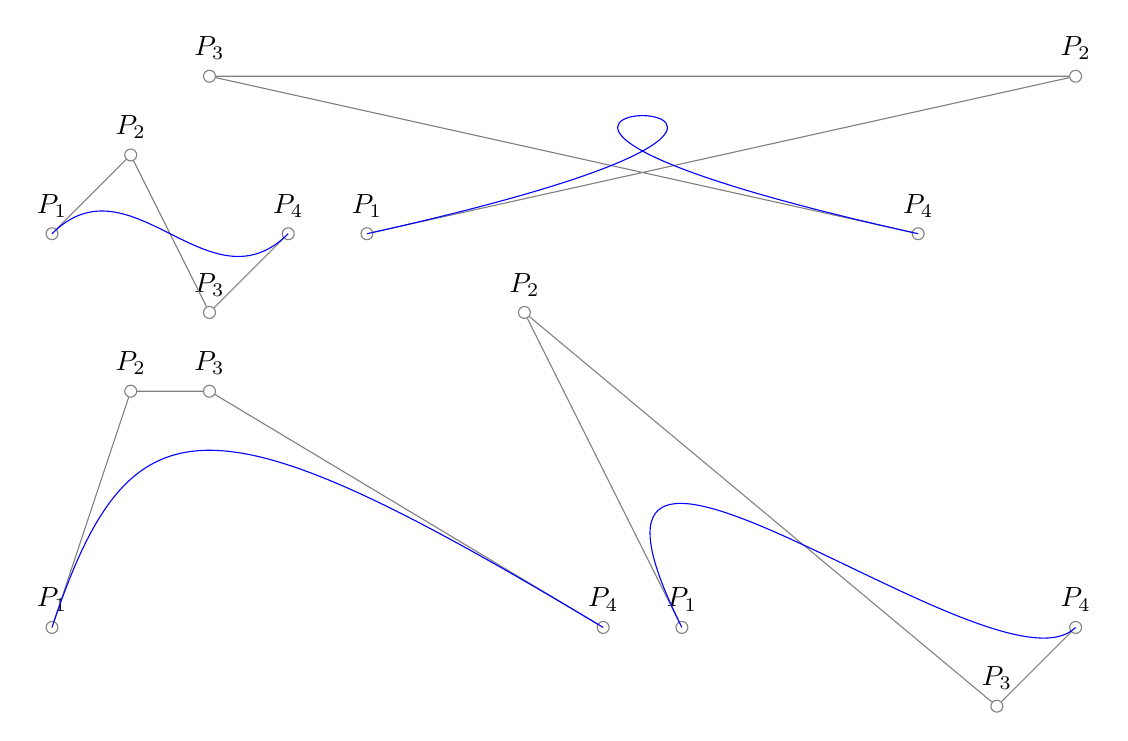
\begin{tikzpicture}
        \Bezier{0,0}{1,1}{2,-1}{3,0}
        \begin{scope}[xshift=4cm]
            \Bezier{0,0}{9,2}{-2,2}{7,0}
        \end{scope}
        \begin{scope}[yshift=-5cm]
            \Bezier{0,0}{1,3}{2,3}{7,0}
    \end{scope}
    \begin{scope}[xshift=8cm,yshift=-5cm]
        \Bezier{0,0}{-2,4}{4,-1}{5,0}
    \end{scope}
\end{tikzpicture}
\caption{Courbes B-splines}
\label[figure]{fig:bsplines}
\end{figure}
\begin{lemme}
    \label{lem:bspline_fermee}
    Soit $\mathcal{C}=(U,P,d)$ une courbe B-Spline.
    Alors, $\mathcal{C}$ est une courbe fermée si et seulement si :
    \begin{enumerate}
        \item $\mathbf{P}_0=\mathbf{P}_m$, où $m=ord(P)$,
        \item $U$ est un vecteur de noeuds uniforme.
    \end{enumerate}
\end{lemme}

\begin{corollaire}
    \label{cor:1}
    Soient $m, N>0$ et $v=(\mathbf{v}_{i,k})_{(i,k)\in\intervalle{0}{m}\times\intervalle{0}{N}}\in\mathcal{M}_{m+1,N+1}(\R^2)$\\
    Soit $\mathcal{C}_0=(U,P^{(0)},d)$ et $\mathcal{C}_k=(U,P^{(k)},d)$, $k\in\NN$, deux courbes B-Splines telles que :
    \begin{enumerate}
        \item $\forall k\in\intervalle{0}{N},\forall i\in\intervalle{0}{m},\, \mathbf{P} _i^{(k)}=\mathbf{P} _i^{(0)}+\mathbf{v}_{i,k}$, 
        \item $U$ est un vecteur de noeuds uniforme.
    \end{enumerate}
\end{corollaire}

\newpage
\subsection{Morphing de courbes B-splines}
\paragraph{Principe} Notre approche se distingue en deux phases. Premièrement, laisser à l'utilisateur le soin de réaliser
l'ajout de points de contrôles, et subséquemment, l'ajustement de la courbe qui modélise la forme souhaitée. Ensuite, nous procédons
au calcul des fonctions de base $B_{i,p}(u)$ ainsi qu'aux points de la courbes $C(u)$ pour l'image source. Ce faisant, en réalisant
une interpolation linéaire des points de controles entre les polygones de contrôles de l'image source et de l'image destination,
nous sommes en mesure de déterminer pour chaque image intermédiaire $0\leq k\leq N$ la position $C^{(k)}(u)$ de la courbe en utilisant
le corollaire \ref{cor:1}.
\subsubsection{Calcul d'une courbe B-spline}
\paragraph{Calcul de la courbe} Dans le sous-domaine mathématique de l'analyse numérique, l'algorithme de de Boor \cite{sheneGeometryNotes} est un algorithme polynomial 
et numériquement stable pour évaluer les courbes splines sous forme de B-splines. 
Il s'agit d'une généralisation de l'algorithme de de Casteljau pour les courbes de Bézier. 
Cet algorithme a été conçu par le mathématicien germano-américain Carl R. de Boor. 
Des variantes simplifiées et potentiellement plus rapides de l'algorithme de de Boor ont été créées, mais elles souffrent d'une stabilité comparativement plus faible.
\begin{algorithm}[h!]
    \BlankLine
    \SetKwFunction{FMain}{calculerPoint}
    \SetKwProg{Fn}{Fonction}{:}{}
    \Fn{\FMain{$u$, $controlPoints$, $nodeVector$}}{
        $k \leftarrow trouverIntervalle(u, nodeVector)$\;
        $d \leftarrow controlPoints.subList(k - deg, k + 1)$\;
        
        \BlankLine
        \tcp{Algorithme de De Boor}
        \For{$r \leftarrow 1$ \KwTo $deg$}{
            \For{$j \leftarrow k$ \KwTo $k - r$ \KwBy $-1$}{
                $i \leftarrow j - k + deg$\;
                $a \leftarrow \frac{u - nodeVector.get(j)}{nodeVector.get(j + deg - r + 1) - nodeVector.get(j)}$\;
                $interpolated \leftarrow d.get(i - 1).nextPoint(d.get(i), a)$\;
                $d.set(i, interpolated)$\;
            }
        }
        
        \BlankLine
        \Return{$d.get(deg)$}\;
    } 
    \caption{Calcul courbes B-splines}
    \label{algo:deboor}
\end{algorithm}
\paragraph{Remarque. } On donne le pseudo-code de la fonction \texttt{trouverIntervalle} dans l'algorithme \ref{algo:trouver-intervalle} en annexe.

\paragraph{Algorithme} On donne ci-après l'algorithme principal pour le morphing de courbes B-splines, basé sur l'approche évoquée plus haut. Malheureusement,
faute d'appréciation, nous n'avons pas pu tester l'algorithme. Nous en donnons une implémentation en Java complète dans les sources du projet. Par ailleurs,
 la javadoc est disponible pour une meilleure compréhension de l'implémentation.
\begin{algorithm}[h!]
    \SetKwInOut{Input}{Entrée}
    \SetKwInOut{Output}{Sortie}
    
    \Input{Les points de contrôle de l'image source $sourcePoints$, les points de contrôle de l'image destination $destinationPoints$, le nombre d'images intermédiaires à générer $numFrames$}
    \Output{Une liste d'images intermédiaires représentant le morphing de courbes B-splines}
    
    \BlankLine
    \tcp{Vérifier que les listes de points de contrôle ont la même taille}
    \If{$sourcePoints.size() \neq destinationPoints.size()$}{
        \Return{$null$}\;
    }
    
    \BlankLine
    \tcp{Calculer les vecteurs de noeuds pour les courbes source et destination}
    $sourceNodeVector \leftarrow calculerNodeVector(sourcePoints.size(), deg)$\;
    $destinationNodeVector \leftarrow calculerNodeVector(destinationPoints.size(), deg)$\;
    
    \BlankLine
    \tcp{Générer les images intermédiaires}
    $intermediateImages \leftarrow$ une liste vide\;
    \For{$i \leftarrow 0$ \KwTo $numFrames$}{
        $t \leftarrow \frac{i}{numFrames}$\;
        
        \BlankLine
        \tcp{Calculer les points de contrôle intermédiaires par interpolation linéaire}
        $intermediatePoints \leftarrow$ une liste vide\;
        \For{$j \leftarrow 0$ \KwTo $sourcePoints.size()$}{
            $sourcePoint \leftarrow sourcePoints.get(j)$\;
            $destinationPoint \leftarrow destinationPoints.get(j)$\;
            $x \leftarrow (1 - t) \cdot sourcePoint.getX() + t \cdot destinationPoint.getX()$\;
            $y \leftarrow (1 - t) \cdot sourcePoint.getY() + t \cdot destinationPoint.getY()$\;
            $intermediatePoints.add(new Point(x, y))$\;
        }
        
        \BlankLine
        \tcp{Calculer les points de la courbe B-spline intermédiaire}
        $intermediateCurve \leftarrow$ une liste vide\;
        \For{$u \gets 0$ \KwTo $1$ \KwBy $0.01$}{
            $point \leftarrow calculerPoint(u, intermediatePoints, sourceNodeVector)$\;
            $intermediateCurve.add(point)$\;
        }
        
        \BlankLine
        \tcp{Ajouter l'image intermédiaire à la liste}
        $intermediateImage \leftarrow genererImage(intermediateCurve)$\;
        $intermediateImages.add(intermediateImage)$\;
    }
    
    \BlankLine
    \Return{$intermediateImages$}\;
    \caption{Morphing de courbes B-splines}
    \label{algo:mainalgorithm}
\end{algorithm}


\section{Morphing d'images quelconques}
\label{sec:morphing_images}

\paragraph{} Après avoir abordé la morphose dans des cas simples, notamment celui de formes unies simples et courbes, 
nous allons désormais nous intéresser à la morphose d'images quelconques. De ce fait, l'objectif à atteindre est de pouvoir
passer d'une image à une autre de manière fluide, en conservant les caractéristiques de chacune des images, tout en \important{évitant l'effet juxtaposition}.

\begin{figure}[h!]
    \centering
    \begin{subfigure}{0.4\textwidth}
        \centering
        \includegraphics[width=0.8\linewidth]{img/p3/lena.png}
        \caption{Image de départ}
        \label{fig:lena}
    \end{subfigure}
    \begin{subfigure}{0.4\textwidth}
        \centering
        \includegraphics[width=0.8\linewidth]{img/p3/lena2.png}
        \caption{Image d'arrivée}
        \label{fig:lena2}
    \end{subfigure}
    \caption{Paires d'images à morpher \cite{beier1992feature}}
\end{figure}

\paragraph{} Pour ce faire, nous allons nous appuyer sur les travaux de Beier-Nelly \cite{beier1992feature}, qui proposent une méthode de morphing basée sur la paramétrisation de l'image
par des vecteurs de contrôle. Ainsi, chaque pixel de l'image est repéré par une association de positions relatives à ces vecteurs de contrôle. En conséquence de quoi, pour deux images
différentes ayant le même nombre de vecteurs de contrôle, il est possible d'associer chaque pixel de l'une, à un pixel de l'autre (ceci ne signifie pas qu'il existe une bijection entre les pixels des deux images). 

\paragraph{Principe} Le principe de la morphose entre deux images repose sur deux étapes majeures. 
La première consiste à déformer les images de départ et d'arrivée, et la seconde à interpoler les images résultantes.
Ce faisant, il nous est possible d'éviter l'effet de superposition des images. Naturellement, plus le nombre de vecteurs de 
contrôle est élevé, plus la morphose sera précise. De même, un grand nombre d'images intermédiaires permettra d'obtenir
 une animation plus naturelle.

\begin{figure}[h!]
    \centering
    \includegraphics[width=0.8\linewidth]{img/p3/principe.png}
    \caption{Calcul d'un image intermédiaire \cite{CSC320W}}
    \label{fig:morphInter}
\end{figure}

\begin{codeb}
Sur la figure \ref{fig:morphInter}, on peut observer le calcul d'une image intermédiaire \emph{Morph}. 
Explicitement, on a : \couleur{$Morph = (1 - \alpha) \times Wrap_0 + \alpha \times Wrap_1$}, où $\alpha$ est un paramètre variant de 0 à 1.
\end{codeb}

\subsection{Déformation des images}
\label{subsec:deformation}
\subsubsection{Préliminaires}
\begin{definition}
    Soient $P$ une image. On note $w$ sa largeur et $h$ sa hauteur, ainsi que $\mathcal{D}(P)=[0,w]\times[0,h]$.
    On appelle \important{vecteur de contrôle} de $P$ tout couple de points du plan $c=(c_1,c_2)$ tel que $c\in\mathcal{D}(P)$.
\end{definition}

\begin{definition}
    Soient $P$ et $Q$ deux images, ainsi que $p$ et $q$ deux vecteurs de contrôle de respectivement $P$ et $Q$. On définit la
    relation $\sim$ telle que $p \sim Q$ si et seulement si $p$ et $q$ sont appariés. Id est, $p$ et $q$ 
    sont une seule et même entité, mais dans deux contextes (\emph{images}) différents.
\end{definition}
\begin{coder}
    \textbf{Conditions.  } Considérons deux images $P$ et $Q$ à morpher en $N>0$ étapes. 
     Alors, chacune possède $n+1$ vecteurs de contrôle $p_{0},\dots,p_{n}$ et $q_{0},\dots,q_{n}$ tels que pour tout $i \in \{0,\dots,n\}$, $p_{i} \sim q_{i}$.

\end{coder}
\subsubsection{Cas simple: un seul vecteur de contrôle}
\begin{definition}
    Soient $P$ et $Q$ deux images, ainsi que $p$ et $q$ des vecteurs de contrôle de resp. $P$ et $Q$.


\end{definition}
\begin{figure}[h!]
    \centering
    \includegraphics[width=0.8\linewidth]{img/p3/uv.png}
    \caption{Apparaiement à un seul vecteur \cite{beier1992feature}}
    \label{fig:deformation}
\end{figure}
\section{Analyse et conception}
On fait suivre sur les pages suivantes les différents diagrammes.
\subsection{Diagramme de cas d'utilisation}


Avant tout projet, un diagramme de cas d'utilisation permet de bien se rendre compte des besoins utilisateurs pour ne pas oublier certaines fontionnalités. Ce diagramme est général, il convient donc aux trois exercices du sujet.

\subsection{Diagramme de classe}

Pour pouvoir implémenter nos classes en Java, il est plus que nécessaire de concevoir un diagramme de classe.

\subsection{Diagramme d'activité}
Un diagramme d'activité est aussi intéressant pour comprendre le focntionnement de l'application.

\includepdf[pages={1},fitpaper=true, pagecommand={},]{/home/cytech/Desktop/Morphing/Morphing/rapport/img/diag/MorphingApp-1.pdf}
\includepdf[pages={1},fitpaper=true, pagecommand={}]{/home/cytech/Desktop/Morphing/Morphing/rapport/img/diag/Diagramme_vierge-1-1.pdf}
\includepdf[pages={1},fitpaper=true, pagecommand={}]{/home/cytech/Desktop/Morphing/Morphing/rapport/img/diag/Diagramme_dactivites.pdf}
\includepdf[pages={1},fitpaper=true, pagecommand={}]{/home/cytech/Desktop/Morphing/Morphing/rapport/img/diag/Diagramme_dactivites.pdf}







Testing
Le testing a été une partie cruciale de notre projet de morphing. Assurer la fiabilité et la précision des algorithmes que nous avons développés nécessitait une approche rigoureuse et méthodique du test. Nous avons mené une série de tests approfondis pour vérifier la robustesse de notre code et garantir que chaque composant fonctionnait comme prévu.
Approche et Méthodologie
Pour tester efficacement notre projet, nous avons adopté une approche en plusieurs étapes :
Tests Unitaires :
Nous avons commencé par des tests unitaires pour chaque fonction individuelle. Cela comprenait toutes les fonctions des classes Line, Point, Couple, etc. Les tests unitaires visaient à vérifier que chaque fonction de chaque classe renvoyait les résultats attendus pour un ensemble donné d'entrées. Des cas de test simples et complexes ont été utilisés pour s'assurer que les fonctions géraient correctement toutes les situations, y compris les cas limites.
Tests d'Intégration :
Une fois que chaque fonction individuelle a été validée, nous avons procédé aux tests d'intégration. Ces tests visaient à vérifier que les différentes classes interagissaient correctement lorsqu'elles étaient combinées. Par exemple, il fallait vérifier que Line, Couple et Point interagissaient correctement entre eux afin que la classe MorphingApp puisse marcher.
Tests de Régression :
Chaque fois que des modifications ou des améliorations étaient apportées au code, nous avons effectué des tests de régression pour s'assurer que les nouvelles modifications n'introduisaient pas de nouveaux bugs ou n'altéraient pas le comportement existant de l'application.
Validation Visuelle :
Enfin, nous avons utilisé des tests visuels pour valider les résultats du morphing. En visualisant les transformations et les courbes générées, on a pu s'assurer que les algorithmes fonctionnaient correctement et produisaient les résultats attendus. Ces tests étaient particulièrement importants pour les aspects visuels du projet, où les erreurs peuvent souvent être détectées plus facilement par l'œil humain.

Les classes des tests peuvent être trouvées en annexe.
Conclusion
Grâce à une approche méthodique et rigoureuse du testing, nous avons pu garantir que notre projet de morphing était fiable, robuste et performant. Les tests ont joué un rôle crucial dans l'assurance qualité et ont permis de livrer un produit final de haute qualité.

\section{Bilans personnels}
\subsection{Bilan Rubens}

Ce projet m'a permis de beaucoup gagner en expérience sur de nombreux aspects, notamment concernant la création d'application Javafx, ainsi que l'arrangement du code avec la méthode PAC. J'ai eu l'impression de bien plus en apprendre sur Java en général avec un réel projet qui permettait de mettre en application toutes les connaissances (mélangé avec des mathématiques), plutôt qu'avec les différents TPs. Également, travailler avec des gens que l'on connaît peu est une expérience dont j'avais peu l'habitude et qui sera importante plus tard, donc je pense que c'était une bonne idée, bien que déplaisante au départ. 
Finalement, je trouve que ce projet s'est révélé très intéressant, enrichissant et amusant.
\subsection{Bilan Alex}

Ce projet fut l'occasion de mettre en pratique nos compétences acquises tout au long de cette première année en cycle ingénieur. J'ai pu comprendre profondément l'utilité de l'étape de conception d'un projet avec les différents diagrammes à concevoir pour ne pas se perdre dans le code. De plus, j'ai appris à utiliser GitHub qui est un outil dont on m'avait déjà beaucoup parlé mais que je n'ai jamais utilisé. Sa prise en main a été assez difficile pour moi au début, car j'aime comprendre exactement ce que je fais et ne connaissant pas cette application, j'ai dû me lancer dans un projet sans connaître parfaitement la prise en main de GitHub.

Néanmois, la partie la plus importante et intéressante selon moi est l'organisation d'un groupe de travail. En effet, durant mes deux années de classe préparatoire aux grandes écoles, le travail de groupe n'était pas du tout mit en avant. Ainsi, avec ce projet, j'ai pu voir la difficulté de travailler avec des personnes qui n'ont pas les mêmes idées, les mêmes manières de penser, les mêmes manières de coder... J'ai donc beaucoup appris sur cet aspect là et j'en garde une très belle expérience.


\subsection{Bilan Paul}
Le projet de morphing a été une expérience extrêmement enrichissante pour moi. J'ai pu approfondir mes connaissances en algorithmes, notamment en travaillent sur l'algorithme de Beier-Neely pour faire du morphing d'images et des transformations géométriques, tout en mettant en pratique des concepts théoriques complexes. Travailler en groupe a également été très bénéfique; j'ai appris différentes méthodes de programmation grâce aux contributions variées de mes coéquipiers, ce qui a enrichi mes compétences et ma perspective sur la résolution de problèmes.

\subsection{Bilan Romain}
J'ai trouvé ce projet très intéressant. Cela m'a permis de mieux comprendre le langage Java ainsi que la partie JavaFx. En effet, nous avons eu des tp sur ceci, mais là nous avons eu la possibilité de voir comment utiliser toutes les fonctionnalités vues en tp dans un projet concret. L'utilisation de la méthode PAC a été plus claire grâce à ce projet. Effectivement, je n'avais pas très bien compris comment celle-ci fonctionnait et grâce à notre travail j'ai finalement compris pourquoi l'utiliser et comment cela fonctionnait. Enfin, le fait de ne pas avoir pu choisir les personnes avec qui nous voulions travailler fut une belle expérience. En effet, je n'en avais pas l'habitude jusque-là et j'ai dû faire face à d'autres manières de penser, d'autres manières de travailler. Cette expérience me sera, j'en suis sur, très bénéfique pour la suite de ma vie étudiante et professionnelle.
\subsection{Bilan Ryan}
Ce projet a été l'occasion pour moi de constater une énième fois les nécessités impérieuses auxquelles je dois faire face, tant dans la gestion d'un groupe, que dans la gestion de mon temps. En effet, j'ai pu constater que la gestion d'un groupe de travail est une tâche ardue, qui nécessite une communication constante, adapté à l'auditoire et, malheureusement, assez répétitive. Autrement, j'ai pu constater que la gestion de mon temps est un aspect que je dois améliorer, car j'ai souvent été attentiste dans les situations requérant la finalisation du travail d'autrui, ce qui ne m'a pas permis d'aboutir le projet en totalité. 

%%%%%%%%%%%%%%%%%%%%%%%%%%%%%
%       Liste des Algos     %
%%%%%%%%%%%%%%%%%%%%%%%%%%%%%
\newpage
\listofalgorithms
%%%%%%%%%%%%%%%%%%%%%%%%%%%%%
%       Liste des figures   %
%%%%%%%%%%%%%%%%%%%%%%%%%%%%%
\newpage
\listoffigures

%%%%%%%%%%%%%%%%%%%%%%%%%%%%%
%           Annexe          %
%%%%%%%%%%%%%%%%%%%%%%%%%%%%%
\newpage
\appendix  % Début des annexes
\appendixpage  % Page de titre pour les annexes
\addappheadtotoc  % Ajouter la page des annexes à la table des matières
\section[Splines]{Morphing de courbes splines}
\begin{algorithm}
    \tcp{Trouve l'intervalle dans le vecteur de noeuds qui contient le paramètre u}
    \SetKwFunction{FMain}{trouverIntervalle}
    \SetKwProg{Fn}{Fonction}{:}{}
    \Fn{\FMain{$u$, $nodeVector$}}{
        $n \leftarrow nodeVector.size() - 1$\;
        \If{$u \geq nodeVector.get(n)$}{
            \Return{$n - 1$}\;
        }
        \For{$i \leftarrow 0$ \KwTo $n - 1$}{
            \If{$u \geq nodeVector.get(i)$ \textbf{and} $u < nodeVector.get(i + 1)$}{
                \Return{$i$}\;
            }
        }
        \Return{$-1$} \tcp{Interval not found}
    }
    \caption{Trouver intervalle}
    \label{algo:trouver-intervalle}
\end{algorithm}
\section{Tests unitaires}
\begin{figure}
    \centering
    \includegraphics[width=1\textwidth]{/home/cytech/Desktop/Morphing/Morphing/rapport/img/testing/test1.png}
    \caption{Résultat des tests unitaires}
    \label{fig:tests1}
\end{figure}
\begin{figure}
    \centering
    \includegraphics[width=1\textwidth]{/home/cytech/Desktop/Morphing/Morphing/rapport/img/testing/test2.png}
    \caption{Résultat des tests unitaires}
    \label{fig:tests2}
\end{figure}
\begin{figure}
    \centering
    \includegraphics[width=1\textwidth]{/home/cytech/Desktop/Morphing/Morphing/rapport/img/testing/test3.png}
    \caption{Résultat des tests unitaires}
    \label{fig:tests3}
\end{figure}
\begin{figure}
    \centering
    \includegraphics[width=1\textwidth]{/home/cytech/Desktop/Morphing/Morphing/rapport/img/testing/test4.png}
    \caption{Résultat des tests unitaires}
    \label{fig:tests4}
\end{figure}
\begin{figure}
    \centering
    \includegraphics[width=1\textwidth]{/home/cytech/Desktop/Morphing/Morphing/rapport/img/testing/test5.png}
    \caption{Résultat des tests unitaires}
    \label{fig:tests5}
\end{figure}
\begin{figure}
    \centering
    \includegraphics[width=1\textwidth]{/home/cytech/Desktop/Morphing/Morphing/rapport/img/testing/test6.png}
    \caption{Résultat des tests unitaires}
    \label{fig:tests6}
\end{figure}
  % Inclusion du fichier d'annexes

%%%%%%%%%%%%%%%%%%%%%%%%%%%%%
%       Bibliographie       %
%%%%%%%%%%%%%%%%%%%%%%%%%%%%%
\newpage
\bibliographystyle{plain}
\bibliography{biblio.bib}
\end{document}
